% (c) 2012 Dimitrios Vrettos - d.vrettos@gmail.com
% (c) 2017 Daniele Zambelli - daniele.zambelli@gmail.com
% 
% Tutti i grafici per il capitolo relativo ai razionali
% 
% 

% Colori per le divisioni:
\def \valposc{green!60!black} % Valore posizionale
\def \quozc{blue!60!black}    % Quoziente
\def \restc{red!60!black}     % Resto


\newcommand{\divisionea}{% divisione 4347:35
\begin{tikzpicture}
\tikzset{node distance=-25ex} 
\begin{scope}[font=\ttfamily]
\matrix (divisione) [matrix of nodes, ampersand replacement=\&]{%
  |[\valposc]|M\&|[\valposc]|C\&|[\valposc]|D\&|[\valposc]|U\\
  4 \& 3 \& 4 \& 7,\& 3 \& 5\\
    \& 8 \& 4 \&   \&
  |[\quozc]|1\&|[\quozc]|2\&|[\quozc]|4,\&|[\quozc]|2\&\\
    \& 1 \& 4 \& 7 \& 
  |[\valposc]|C\&|[\valposc]|D\&|[\valposc]|U\&|[\valposc]|d\\
    \&   \&   \& 7 \& 0\\
    \&   \&   \&   \& |[\restc]|0 \&\\
};
\end{scope}
\draw(divisione-2-5.north west)--(divisione-3-5.south west);
\draw(divisione-3-5.north west)--(divisione-3-8.north east);
\end{tikzpicture}
}

\newcommand{\divisioneb}{% divisione 1523:7
\begin{tikzpicture}
\tikzset{node distance=-25ex} 
\begin{scope}[font=\ttfamily]
\matrix (divisione) [matrix of nodes, ampersand replacement=\&]
{%
  |[\valposc]|M\&|[\valposc]|C\&|[\valposc]|D\&|[\valposc]|U\&
  |[\valposc]|d\&|[\valposc]|c\&|[\valposc] |m\\
  1 \& 5 \& 2 \& 3,\&   \&   \&   \& 7 \& ~ \& ~ \&\&\&\&\&\& ~ \&\\
    \& 1 \& 2 \&   \&   \&   \&   \&
|[\quozc]|2\&|[\quozc]|1\&|[\quozc]|7,\&|[\quozc]|5\&|[\quozc]|7\&
|[\quozc]| 1\&|[\quozc]|4\&|[\quozc]|6\&|[\quozc]|8\&   \&\\
    \&   \& 5 \& 3 \&   \&   \&   \& 
|[\valposc]|C\&|[\valposc]|D\&|[\valposc]|U\&|
[\valposc]|d\&|[\valposc]|c\&|[\valposc]|m\\
    \&   \&   \& 4 \& 0\\
    \&   \&   \&   \& 5 \& 0\\
    \&   \&   \&   \&   \& 1 \& 0\\
    \&   \&   \&   \&   \&   \& 3 \& 0\\
    \&   \&   \&   \&   \&   \&   \& 2 \& 0\\
    \&   \&   \&   \&   \&   \&   \&   \& 6 \& 0\\
    \&   \&   \&   \&   \&   \&   \&   \&   \& |[\restc]|4\\
};
\end{scope}
\draw(divisione-2-8.north west)--(divisione-3-8.south west);
\draw(divisione-2-8.south west)--(divisione-2-16.south east);
\end{tikzpicture}
}

\newcommand{\frazionea}{% parti della frazione
  \disegno{
    \node {$\dfrac{42}{75}$};
    \begin{scope}[\quozc]
    \draw [<-] (1, .5) to [out=0, in=180] (3, 1.5) node [right] 
      {~~~~numeratore};
    \draw [->] (8.5, 1.5) to [out=0, in=180] (10.5, .5);
    \end{scope}
    \begin{scope}[\valposc]
    \draw [<-] (1, 0) -- (3, 0) node [right] {~linea di frazione};
    \draw [->] (8.5, 0) -- (10.5, 0);
    \end{scope}
    \begin{scope}[red!50!black]
    \draw [<-] (1, -.5) to [out=0, in=180] (3, -1.5) node [right] 
      {~~~denominatore};
    \draw [->] (8.5, -1.5) to [out=0, in=180] (10.5, -.5);
    \end{scope}
    \node at (11.5, 0) {$\dfrac{num}{den}$};
  }
}

\newcommand{\addizione}{% addizione algebrica tra frazioni
  \disegno{
    \node {$\dfrac{a}{b} \mp \dfrac{c}{d} \qquad = \qquad
             \dfrac{ad}{bd} \mp \dfrac{bc}{bd} = \dfrac{ad \mp bc}{bd}$};
    \begin{scope}[\quozc]
    \draw [->] (-5.5, 1) node [above right, yshift=3mm] {$\times d$} 
          to [out=45, in=135] (0, 1);
    \draw [->] (-5.5, -1) node [below right, yshift=-3mm] {$\times d$} 
          to [out=-45, in=-135] (0, -1);
    \end{scope}
    \begin{scope}[red!50!black]
    \draw [->] (-4, 1) to [out=45, in=135] (1.7, 1)
          node [above left, yshift=3mm] {$\times b$} ;
    \draw [->] (-4, -1) to [out=-45, in=-135] (1.7, -1)
          node [below left, yshift=-3mm] {$\times b$} ;
    \end{scope}
  }
}

\newcommand{\reciproco}{% reciproco di una frazione.
  \disegno{
    \node {$\dfrac{a}{b}$};
    \begin{scope}[\quozc]
    \path [postaction={decoration={text along path, text={reciproco},
           text align={align=center}}, decorate}] 
          (1, 0.2) to [out=45, in=180] (3, 0.8) to [out=0, in=135] (5, 0.2);
    \draw [<->] 
          (1, 0) to [out=45, in=180] (3, 0.6) to [out=0, in=135] (5, 0) 
;
    \end{scope}
    \node at (6, 0) {$\dfrac{b}{a}$};
  }
}

\newcommand{\rettafra}{% 
  % Frazioni rappresentate sull'asse
  \disegno[10]{
    \assecontrattini{-6}{+6.3}{0}{}
    \foreach \x in {-6, -5, -4, -3, -2, -1, 0, +1, +2, +3, +4, +5, +6}{
      \draw  (\x, 0) [below, font=\small] node {$\x$};
    }
    \foreach \x/\l in {0.25 / $\frac{1}{4}$, 
                       0.5 / $\frac{1}{2}$, 
                       0.75 / $\frac{3}{4}$, 
                       1.33 / $\frac{4}{3}$,
                       1.66 / $\frac{5}{3}$,
                       2 / $\frac{6}{3}$,
                       2.5 / $\frac{5}{2}$, 
                       3.5 / $\frac{7}{2}$, 
                       4.8 / $\frac{24}{5}$, 
                       5.2 / $\frac{26}{5}$,  
                       -1.33 / $-\frac{4}{3}$,
                       -2.5 / $-\frac{5}{2}$,
                       -3.66 / $-\frac{1}{3}$,
                       -4.5 / $-\frac{9}{2}$,
                       -5.66 / $-\frac{17}{3}$}{
      \draw [latex-] (\x, 0) -- (\x, 0.3) node [above] {\l};
    }
  }
}

\newcommand{\rettarazese}{% 
  % Frazioni rappresentate sull'asse
  \disegno[20]{
    \asse{(-3.3, 0)}{(3.3, 0)}{}{}  %{-3.1}{+3.1}{0}{}
    \foreach \x in {-3.1, -3, ..., +3.2}{
      \draw (\x, +.05) -- (\x, 0);
    }
    \foreach \x in {-3.2, -3, ..., +3.2}{
      \draw (\x, +.1) -- (\x, 0);
    }
    \foreach \x in {-3, -2, -1, 0, +1, +2, +3}{
      \draw (\x, +.1) -- (\x, -.1) [below, font=\small] node {$\x$};
    }
    \foreach \x in {-2.5, -2.2, -1.5, -1.2, -0.6, -0.4, 
                    +.2, +.7, +1.2, +1.5, +1.8, +2.5, +2.4}{
      \filldraw [fill=blue](\x, 0) circle(1.5pt);
    }
  }
}

\newcommand{\frazdeca}{
\disegno{
  \tikzset{node distance=-25ex} 
  \begin{scope}[font=\ttfamily]
  \matrix (divisione) [matrix of nodes, ampersand replacement=\&]
        {%
  1 \& 9 \& 7 \& 8\\
    \& 3 \& 7 \&|[blue]|2\&|[blue]|4,\&|[blue]|6\&|[blue]|2\&|[blue]|5\\
    \&   \& 5 \& 0\\
    \&   \&   \& 2 \& 0\\
    \&   \&   \&   \& 4 \& 0\\
    \&   \&   \&   \&   \& $=$\\
        };
    \end{scope}
    \draw (divisione-1-4.north west)--(divisione-2-4.south west);
    \draw (divisione-2-4.north west)--(divisione-2-8.north east);
    \node [left=of divisione-2-8.north west, yshift=-5mm] 
          {$\dfrac{197}{8} = 28,625$};
  }
}

\newcommand{\frazdecb}{
\disegno{
  \tikzset{node distance=-25ex} 
  \begin{scope}[font=\ttfamily]
  \matrix (divisione) [matrix of nodes, ampersand replacement=\&]
% 
% \begin{tikzpicture}[node distance=-25ex]
%   \begin{scope}[font=\ttfamily]
%     \matrix (divisione) [matrix of nodes]
      {%
 1 \& 5 \& 5 \& 1 \& 2\\
   \& 3 \& 5 \&|[blue]|1\&|[blue]|2,\&|[blue]|9\&|[blue]|1\&|[blue]|6\\
   \& 1 \& 1 \& 0\\
   \&   \&   \& 2 \& 0\\
   \&   \&   \&   \& 8 \& 0\\
   \&   \&   \&   \&   \& 8\\
      };
  \end{scope}
  \draw(divisione-1-4.north west)--(divisione-2-4.south west);
  \draw(divisione-2-4.north west)--(divisione-2-8.north east);
  \node [left=of divisione-2-8.north west, yshift=-5mm] 
        {$\dfrac{155}{12} = 12,91\overline{6}$};
}
}

\newcommand{\sottrazioneraz}{
\disegno{
  \tikzset{node distance=-25ex} 
  \begin{scope}[font=\ttfamily]
  \matrix (divisione) [matrix of nodes, ampersand replacement=\&]
% 
% \begin{tikzpicture}[node distance=-25ex]
%   \begin{scope}[font=\ttfamily]
%     \matrix (divisione) [matrix of nodes]
      {%
$1000n~=$\& 1 \& 4 \& 3 \& 5 \& 6, \& 5 \& 6 \& 5 \& 6 \& 5 \& 6 
\& 5 \& 6 \& \dots \&$-$\\
$~~10n~=$\&   \&   \& 1 \& 4 \& 3, \& 5 \& 6 \& 5 \& 6 \& 5 \& 6 
\& 5 \& 6 \& \dots \&$=$\\
$~990n~=$\& 1 \& 4 \& 2 \& 1 \& 3, \& 0 \& 0 \& 0 \& 0 \& 0 \& 0 
\& 0 \& 0 \& \dots \& ~\\
      };
  \end{scope}
  \draw(divisione-3-1.north west)--(divisione-2-16.south east);
}
}

\newcommand{\rett}{
% \begin{tikzpicture}[x=10mm,y=10mm,font=\small]
  \disegno{
    \fill[fill=gray!10] (1, 1) rectangle (5, 10);
    \draw[style=help lines, step=1, dashed, black!20] 
         (-0.2, -0.2) grid (6.2, 11.2);
    \draw (1,1) rectangle (5, 10);
    \node (b) at (3, .5) {$b$};
    \node (h) at (5.5, 5.5) {$h$};
  }
}

\newcommand{\notesp}{
  % Notazione esponenziale sull'asse
  \def \alta{1.6}
  \def \altb{.9}
  \disegno[5]{
    \assecontrattini{-14}{+14}{0}{\Q}
    \draw (0, \alta) node [above=3mm] {\large $\alpha = a \cdot 10^n$};
    \begin{scope}[thin, font=\small]
      \draw [below] (0, 0) node {$0$};
      \draw [above] 
            (-1, 0) node {$-1$} (+1, 0) node {$+1$}
            (-10, 0) node {$-10$} (+10, 0) node {$+10$};
      \draw (0, 0) -- (0, \alta) 
            (-1, 0) -- (-1, -\alta) (+1, 0) -- (+1, -\alta)
            (-10, 0) -- (-10, -\alta) (+10, 0) -- (+10, -\alta);
      \draw [-latex] (0, \altb) -- 
            node [midway, above] {$a < 0$} (-13, \altb);
      \draw [-latex] (0, \altb) -- 
            node [midway, above] {$a > 0$} (+13, \altb); 
      \draw [latex-latex] (-1, -\altb) -- 
            node [midway, below] {$n < 0$} (+1, -\altb);
      \draw [-latex] (-10, -\altb) -- 
            node [midway, below] {$n > 0$} (-13, -\altb);
      \draw [-latex] (+10, -\altb) -- 
            node [midway, below] {$n > 0$} (+13, -\altb);
      \draw [-latex] (-10, -\altb) -- 
            node [midway, below] {$n = 0$} (-1, -\altb);
      \draw [-latex] (+10, -\altb) -- 
            node [midway, below] {$n = 0$} (+1, -\altb);
    \end{scope}
  }
}

\newcommand{\esempiosegmenti}[2]{
  % Somma di segmenti
  \def \num{#1}
  \def \den{#2}
  \def \alta{.6}
  \def \altb{.4}
  \disegno[7]{
%     \draw [ultra thick, violet!70!black] (0, 0) -- (\den, 0);
    \foreach \x in {0, ..., \num}{\draw (\x, +\alta) -- (\x, -\alta);}
    \foreach \x in {\num, ..., \den}{\draw (\x, +\alta) -- (\x, \alta-.4);}
    \draw (.5, 0) node  {$x$};
    \begin{scope}[thin, font=\small]
%       \draw (0, 0) -- (0, \alta) (\den, 0) -- (\den, \alta) 
%             (0, 0) -- (0, -\alta) (\num, 0) -- (\num, -\alta);
      \draw [ultra thick, violet!70!black] (0, +\altb) -- 
            node [midway, above] {$a$} (\den, +\altb);
      \draw [ultra thick, violet!70!black] (0, -\altb) -- 
            node [midway, below] {$b$} (\num, -\altb);
    \end{scope}
  }
}

\newcommand{\horus}{
% (c) 2012 Dimitrios Vrettos - d.vrettos@gmail.com
% horus
% Occhio di Horus 
\pgfdeclareimage[interpolate=true]{eye}{\folder img/eye.png}
%{\folder img/eye.pdf}
\begin{tikzpicture}[scale=.7]
    \pgftext[at=\pgfpoint {0mm}{0mm},left,base]{\pgfuseimage{eye}}
    \node (a) at (10mm,65mm) {$\frac{1}{2}$};
    \node (b) at (30mm,65mm) {$\frac{1}{8}$};
    \node (c) at (50mm,65mm) {$\frac{1}{16}$};
    \node (d) at (10mm,0mm) {$\frac{1}{64}$};
    \node (e) at (30mm,0mm) {$\frac{1}{4}$};
    \node (f) at (50mm,0mm) {$\frac{1}{32}$};
  \begin{scope}[->,color=gray, thick]
    \draw (a)--(19mm,34mm);
    \draw (b)--(29mm,54mm);
    \draw (c)--(40mm,35mm);
    \draw (d)--(19mm,14mm);
    \draw (e)--(29mm,35mm);
    \draw (f)--(41mm,16mm);
  \end{scope}
\end{tikzpicture}
}

\newcommand{\frazioneb}{
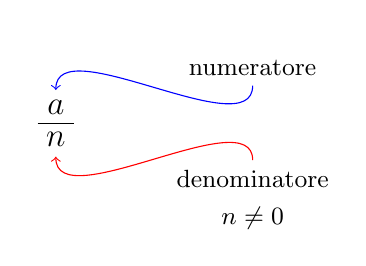
\begin{tikzpicture}
  \begin{scope}[font=\large]
    \matrix (frazione)  at (0,0){%
      \node (num) {$a$};\\
      \node (den) {$n$};\\
    };
  \end{scope}

  \draw (num.south west)--(num.south east);

  \begin{scope}[font=\small]
    \node (testo1) at (25mm,7mm) {numeratore};
    \node (testo2) at (25mm,-7mm) {denominatore};
    \node (testo3) at (25mm,-12mm) {$n\neq0$};
  \end{scope}

  \draw[->,blue] (testo1) .. controls +(down:10mm) and +(up:10mm) .. (num) ;
  \draw[->,red] (testo2) .. controls +(up:10mm) and +(down:10mm) .. (den) ;
\end{tikzpicture}
}
